\cotefile{77}

\scanpage{98}

Considérons alors

\[
t'=\tilde f(x\unsure{+|-}iy)=x\wedge y/q(x)=x\wedge y
\]

il est orth. à $F$, \inserted{et partout non nul} donc $t$ de la forme $t=\lambda t'$, de plus $q(t)=q(\lambda t')=-1$, donc $\lambda^2=1$. \deleted{Considérons}

\deleted{Donc \unsure{alors}}

\[
\left\{\begin{aligned} &q(x)=q(\lambda y)=1,\quad\varphi(x,\lambda y)=0\\ &\deleted{\unsure{x+iy|x+i\lambda y}}\tilde f(x+i\lambda y)=x\wedge\lambda y=\lambda x\wedge y=\lambda t'=t \qquad\text{O.K.}\\ &\deleted{f(x+i\lambda y)=}\end{aligned}\right.
\]

\uline{Corollaire} En inversant l'iso. $f$, on trouve une inclusion ouverte (en car. rés. $\ne 2$)

\[
\Sigma\lhook\joinrel\xrightarrow{g}X^{S[i]}\tag*{(24)}
\]

\deleted{\uline{Remarque} Soit $q'=-q$, on a}

\[
\deleted{\delta(q')=-\delta(q)=\omega^{\otimes(-2)}}
\]

\deleted{donc $(E,q',\omega)$ est \deleted{\unsure{anti}}\inserted{structure} spéciale-orthogonale au sens modifié, forme bil. associée}

\[
\deleted{\varphi'(x,y)=-\varphi(x,y)}
\]

\deleted{Si on calque la définition de \inserted{$[\,,\,]=$}$[\,,\,]_q$ pour $q'$, on trouve $[\,,\,]_{q'}=[\unsure{{}^{\prime}},\,]'$ défini par}

\[
\deleted{\varphi'([x,y]',z)\,\omega=2x\wedge y\wedge z}
\]

\deleted{i.e.}

\[
\deleted{\varphi(\unsure{{}^{\prime\prime}}[x,y],z)\,\omega=-\varphi'([x,y],z)\,\omega}
\]

\[
\deleted{[x,y]'=-[x,y].}
\]

\deleted{La formule (21) devient alors}

\[
\deleted{q'([x,y]')=4q'(x)q'(y)\underbrace{\sin^2(\widehat{x,y}\,')}_{1-\deleted{\unsure{4}}\varphi'(x,y)^2/4q'(x)q'(y)}}\tag*{(25)}
\]

% archive sheet number: 97
\scanpage{99}

Notons qu'on a une immersion canonique

\[
X\lhook\joinrel\longrightarrow X^{S[i]}
\]

qui ici s'explicite à partir de

\[
\begin{aligned}\tilde X&\longrightarrow\tilde X^{S[i]}\\ x&\longmapsto x+\underline i\,0\end{aligned}
\]

\deleted{\uline{Lemme} Soit $\unsure{\zeta|z|\xi}=x+iy\in\Gamma\tilde X^{S[i]}$, \inserted{i.e. $q(x)=q(y)$, $\varphi(x,y)=0$ $x+\underline i y$ partout non nul} Pour que $\zeta\in\Gamma\tilde U$ i.e. $q(x)=q(y)\in\Gamma G_m$, il f. et s. que $\exists\,\alpha=a+ib\in\deleted{\unsure{G}}\Gamma G_m^{S[\underline i]}$ \inserted{$(a^2+b^2\in\Gamma G_m)$} et $x_0\in\Gamma\tilde X$ ($q(x_0)=0$ $x_0$ \unsure{non nul en} tte fibre \unsure{\ldots}) tels que $\zeta=\alpha x_0$ i.e.}

\[
\deleted{x=ax_0,\ y=bx_0}
\]

En \deleted{fait} on trouve que

\uline{Proposition} L'application inverse de $f:\inserted{U\xrightarrow{\sim}\Sigma}$ (\unsure{déduit|déduite} par passage au quotient de $\tilde f:\tilde U\to\Sigma$, $\tilde f(x+iy)=[x,y]/q(x)$) induit un isomorphisme

\[
\boxed{\Sigma\xrightarrow{\sim}\tilde X^{S[i]}-\tilde X=U}
\]

Ceci équivaut au \deleted{lemme}

\uline{Lemme} Si $S=\operatorname{Spec} k$, $k$ un corps, \inserted{alg clos de car $\ne 2$} alors pour \deleted{\unsure{que}} $x+\underline i y\in\Gamma\tilde X^{S[i]}$ [$x,y$ deux él. de $E$ \inserted{non nuls tous deux} tels que \deleted{$x,y$} \deleted{\unsure{non coll. ou|non colin., soit}, $a+ib$ \unsure{ou non} tels que} \inserted{l'un \unsure{au|ou} \unsure{moins}} i.e. $y=\lambda x$, \deleted{\unsure{ou ait} \unsure{$x\ne0$}} \inserted{avec} $\lambda^2\ne-1$, \inserted{et $q(x)=q(y)$, $\varphi(x,y)=0$}] \deleted{\unsure{soit|alors}} \unsure{;|,} on a $x+iy\notin\tilde U^{\deleted{\unsure{S[i]}}}$ i.e. $q(x)=q(y)=0$ sss $x+\underline i y=(a+\underline i b)x_0$, avec $x_0\in\Gamma\tilde X$ i.e. $\unsure{\cdot}x_0\in E^{*}$, $q(x_0)=0$, \deleted{$a+b$} $a+\underline i b\in\Gamma G_m^{S[i]}$ i.e $a^2+b^2\ne0$.

% archive sheet number: 98
\scanpage{100}

En effet, \deleted{on a}\inserted{sachant qu'on a} $y=\lambda x$, \unsure{i.e.} $x+iy=(a+\underline i b)x_0$, \deleted{\unsure{et}} avec $x_0=x$ \inserted{et $a+\underline i b=1+\underline i\lambda$} et on a $a^2+b^2\deleted{\unsure{\ne0}}=1+\lambda^2\ne0$ puisque, on doit avoir $\lambda^2\ne-1$, d'où nécessité. Pour Suffisance, si $x+iy=x_0(a+ib)$, i.e. $x=\deleted{\unsure{q}}ax_0,\ y=by_0$, on aura bien sûr $q(x)=q(y)={\unsure{a}}^{2}q(x_0)=0$

\figure{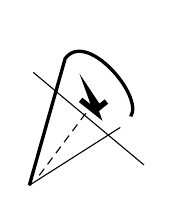
\begin{tikzpicture}[scale=.7]\draw[very thick] (0,0)--(.65,2.3) .. controls (1.04,2.83) and (2.08,1.62) .. (1.84,1.25);\draw (0,0)--(1.65,1.05) (.07,2.05)--(2.08,.37);\draw[densely dashed] (.18,.18)--(1.16,1.49);\draw[line width=2pt] (.93,1.55)--(1.22,1.32)--(1.10,1.65)--(1.26,1.41)--(1.40,1.52);\end{tikzpicture}}

O.K. \ldots

\deleted{\uline{Cas de la car 2} $S[\underline i]$ est alors can. isom. au schém. des \unsure{nbs} duaux, \inserted{$\underline i=1+\varepsilon$ donc} $\deleted{\unsure{\tilde X|X}}X^{S[\underline i]}$ est le fibré tangent à $X$.}

\deleted{On trouve}

\[
\begin{aligned}&\deleted{x+\underline i y=(\underbrace{x+y}_{z})+\varepsilon y\longmapsto[x,y]/q(x)}\\ &\deleted{(x+y\ne0\text{ i.e. }x\ne y)}\qquad\deleted{=[x+y,y]/q(y)}\\ &\deleted{z+\varepsilon y\longmapsto[z,y]/q(y)}\end{aligned}
\]

\[
\deleted{\unsure{\text{à}}\left\{\begin{aligned}&z\ne0\\ &\underbrace{q(y+z)=q(y)\unsure{,}\ne0}_{q(z)\deleted{\unsure{+|=}}\varphi(y,z)}\end{aligned}\right.}
\]

\deleted{\unsure{alors}}

\diagram{\begin{tikzcd}[ampersand replacement=\&,column sep=small,row sep=small] \deleted{\left\{\begin{aligned}\det u&=1\\\operatorname{Tr}u&=0\end{aligned}\right.\;(\Rightarrow u^2+1=0)}\arrow[r,leftrightarrow,"{?}"] \& \deleted{\left\{\begin{aligned}&x+\underline iy\quad q(x)=q(y)\ne0,\ \varphi(x,y)=0\\&\deleted{\unsure{y}}=\lambda\end{aligned}\right.}\\ \deleted{u=\deleted{\unsure{+}}[v,w]/\det v}\arrow[u,Rightarrow,"{?}"'] \& \deleted{\text{où }\left\{\begin{aligned}&\det v=\det w\ne0,\quad\operatorname{Tr}v=\operatorname{Tr}w=0\\ &\operatorname{Tr}vw=0\\ &\deleted{\unsure{k}v,w\ \text{pas de la forme }\lambda v,\ v+\underline i w}.\\ &\deleted{\unsure{v\ne v}}\quad v\ne w\end{aligned}\right.}\end{tikzcd}}

\[
\det[v,w]
\]

% archive sheet number: 99
\scanpage{101}

\deleted{Posons $q''=4q'=-4q$, $\omega''=8\omega$, de sorte que}

\[
\begin{aligned}&\deleted{\delta(q'')=-2^6\delta(q)=2^6\omega^{\otimes2}=(8\omega)^{\otimes2}=\omega''^{\otimes2}}\\&\deleted{\delta(q'')=\omega^{\unsure{\prime\prime}\otimes2}}\end{aligned}
\]

\deleted{La formule (\unsure{15|11|25}) prend la forme}

\[
\deleted{q''(}\tag*{(26)}
\]

\uline{Remarque} Posons

\[
q_\lambda=\lambda q\qquad\varphi_\lambda=\lambda\varphi\qquad [\,,\,]_{\lambda,\mu}=\deleted{\unsure{\tfrac1{\lambda}}}\inserted{(\lambda\mu)^{-1}}[\,,\,],\quad\omega_\mu=\mu\omega
\]

\deleted{La formule (8) s'écrit alors}

\[
\deleted{q_\lambda([x,y]_\lambda)=\lambda}
\]

\[
\deleted{2x\wedge y\wedge z=\varphi_\lambda([x,y]_\lambda,z)\,\omega}
\]

donc on a

\[
\left\{\begin{aligned}&\underline{\delta'(q_\lambda)}\bigl[=\lambda^3\delta(q)=-\underline{\lambda^3}\omega^{\otimes2}\bigr]=\underline{-\lambda^3\mu^{-2}\omega_\mu^{\otimes2}}\\ &\underline{2x\wedge y\wedge z}=\underline{\varphi_\lambda([x,y]_\lambda,z)\,\omega_\mu^{\unsure{3}}}\end{aligned}\right.
\]

\[
\left\{\begin{aligned}q_\lambda([x,y]_{\lambda,\mu})&=\lambda(\lambda\mu)^{-2}q([x,y])=-4\lambda^{-1}\mu^{-2}q(x)q(y)\sin^2(\widehat{x,y})\\ &=-4\lambda^{-3}\mu^{-2}q_\lambda(x)q_\lambda(y)\sin^2(\widehat{x,y})\end{aligned}\right.
\]

On veut choisir $\lambda,\mu$ tels que $-4\lambda^{-3}\mu^{-2}=1$ i.e. $\lambda^{-3}\mu^{-2}=-\frac14$ avec $\lambda,\mu$ des \inserted{(au signe près)} puiss. de 2

\figure{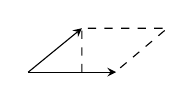
\begin{tikzpicture}[scale=.62,>=stealth]\draw[->] (0,0)--(1.8,0);\draw[->] (0,0)--(1.1,.9);\draw[dashed] (1.1,0)--(1.1,.9)--(2.85,.9)--(1.78,0);\end{tikzpicture}}

\[
\lambda=-2^\alpha,\ \mu=2^\beta\qquad \lambda^{-3}\mu^{-2}=-2^{-(3\alpha+2\beta)}=-2^2
\]

i.e. on veut $3\alpha+2\beta=-2$ p.ex. on prend $\alpha=0$, $\beta=\deleted{\unsure{0|-}}1$ ce qui donne

\[
\lambda=-1,\ \mu=1/2\qquad q_\lambda=\inserted{q'\deleted{\unsure{_\lambda}}}=-q,\quad\omega_\mu=\unsure{2|1}\omega'=\tfrac12\omega
\]

\inserted{$[x,y]_{\lambda,\mu}=[x,y]'=-2[x,y]$}

\[
\left\{\begin{aligned}\delta'(q')&=+4\omega'^{\otimes2}=(2\omega')^{\otimes2}\\ x\wedge y\wedge z&=\tfrac12\varphi'([x,y]',z)\,\omega'\\ q'([x,y]')&=q'(x)q'(y)\sin^2(\widehat{x,y})\\ &=q'(x)q'(x)\bigl(1-\tfrac14\varphi(x,y)^{2}\bigr)\end{aligned}\right.
\]

% archive sheet number: 100
\scanpage{102}

\uline{Car. \unsure{quelc.}}

\[
\deleted{q([x,y])=\varphi(x,y)^2}
\]

\deleted{Donc si $x+\underline i y\in\Gamma\tilde U$, donc $q(x)=q(y)\inserted{\in\Gamma G_m}$, $\varphi(x,y)=0$, alors $q([x,y])=0$. Si on remplace $x+\underline i y$ par $(a+\underline i b)(x+\underline i y)=\underbrace{ax-by}_{x'}+\underline i(\underbrace{bx+ay}_{y'})$, on trouve $x'\wedge y'=(a^2+b^2)x\wedge y$, $q(x')=q(y')=(a^2+b^2)q(x)$, donc $x'\wedge y'/q(x')=x\wedge y/q(x)$. On trouve}

\[
\deleted{\unsure{x+iy}}\quad x+\underline i y\in\Gamma\tilde U\longrightarrow[x,y]/q(x)\in\Sigma_{-4}
\]

donc

\[
\tilde g:\tilde U\longrightarrow\Sigma_{-4}
\]

passe au quotient en

\[
g:U^{\deleted{\unsure{S[i]}}}\longrightarrow\Sigma_{-4}
\]

(\unsure{indépendam$^{\mathrm t}$|indépendamment} de la car.). En car. 2, on a

\deleted{Supposons $[x,y]/q(x)=[x',y']/q^{2}(x)$ ; donc (quitte à se localiser et à remplacer $x'$ par $\lambda x'$). \unsure{supp.} $q(x)=q(x')$, $[x,y]=[x'^{\deleted{\unsure{+}}},y']$. Supposons qu'on \deleted{a) Supposons $y$} \unsure{soit en car.} \unsure{$\ne2$}}

\[
[x,y]=\varphi(x,y)H\quad\text{avec }\left\{\begin{aligned}&H\text{ base du centre de }\unsure{\tilde{\mathfrak g}|\tilde g}\\ &q(H)=1\end{aligned}\right.
\]

donc $q([x,y])=\varphi(x,y)^2$

Si $\varphi(x,y)=0$ (p.ex. $x+\underline i y\in\Gamma\tilde X^{S[i]}\supset\Gamma(\tilde U)$\unsure{\ldots}) on a $[x,y]=0$. Donc en car. 2 l'application $g$ se spécialise en l'application constante de valeur 0 : rien à faire\ldots !

% archive sheet number: 101
\scanpage{103}

\mspage{\fbox{$1'$}}

Soit $S$ schém., $E$ fibré affine de rg 3 sur $S$, $\Sigma\subset E$ une quadrique affine \inserted{(\unsure{projectiv$^{\mathrm t}$} \deleted{régulière}\inserted{lisse})} -- il revient au $=$ de partir d'un fibré projectif \deleted{\unsure{lisse}} $P$\inserted{$(=\hat E)$} de rang 3, d'une quadrique projective \inserted{lisse} $Q$\inserted{$(=\hat\Sigma)$}$\subset P$, et d'un hyperplan $H$ de $P$ -- en prenant $E=P\setminus H$, $\Sigma=Q\cap E=Q\setminus Q\cap H$. \deleted{On}

[Sauf erreur, il revient encore au $=$ de se donner $Q$ comme schéma (projectif lisse) sur $S$ qui soit une forme de $P^1\times P^1$, ce qui détermine $P$ canoniquement, et de prendre un diviseur \inserted{\deleted{\unsure{$Q_1$}}$X$} de type $(1,1)$ sur $Q$ -- lequel sera défini par un $H$ bien déterminé de $P$\ldots]

On suppose que $\Sigma$ n'est pas un paraboloïde, \inserted{sur aucune fibre} i.e. que $H$ n'est pas tangent à $Q$, ou encore que $\deleted{\unsure{C}}X=H\cap Q=\hat\Sigma\setminus\Sigma$ est lisse i.e. un 1-fibré projectif sur $S$. On peut dire aussi que la donnée de $(E,\Sigma)$ équivaut à $E$, \unsure{sa|son} ext. $\unsure{\mathscr E|\mathcal E}$ de $\mathcal O_S$ par

% archive sheet number: 102
\scanpage{104}

un fibré vectoriel de rang 3 $V$ (le fibré des translations de $E$)

\[
0\longrightarrow V\mathbin{\text{---}}\unsure{\mathscr E|\mathcal E}\mathbin{\text{---}}\mathcal O_S\mathbin{\text{---}}1
\]

et ``une'' forme quadratique $Q$ \inserted{lisse} sur $\mathscr E$ définie loc$^{\mathrm t}$ mod \unsure{mult$^{\mathrm n}$|mult.} par une unité [c'est ce que signifie que $\Sigma$ est défini par une fonction polynomiale de degré $\leq2$, et qu'il est \unsure{project$^{\mathrm t}$|projectiv$^{\mathrm t}$} lisse\ldots]

La condition que $\Sigma$ ne soit pas un paraboloïde signifie que $q\mid V$ est \deleted{non dégénérée} lisse. Si les car. résiduelles sont $\ne2$, cela signifie \inserted{aussi} que $\mathscr E=V+V^\perp$, donc $E$ se trouve muni d'une origine $o$ \inserted{permettant de l'identifier à $V$} (le polaire de $H=P(V)$ p.r. à \inserted{la quadrique} $Q$) et $\Sigma$ est stable pour la sym. p.r. à cette origine -- $o$ s'appelle le \uline{centre} de la quadrique affine. Ce centre $o$ \inserted{(section de $E$ sur $S$)} ne rencontre pas $\Sigma$, donc la fonction quadratique peut être normalisée \inserted{loc.} par la condition que sa valeur sur $o$ soit 1 ; ce qui la détermine de

% archive sheet number: 103
\scanpage{105}

façon unique et assure son existence et unicité globales. On \deleted{\unsure{a donc}} trouve alors que sur $\underset{\substack{\Vert\\V\times1}}{E}\deleted{\unsure{=V}}\inserted{\subset\mathscr E}$ la fonction induite par $Q$ est de la forme $q(x)+1$, où $q$ est la forme quadratique \inserted{lisse} induite sur $V$ par $Q$. Donc la donnée de $\Sigma$ dans $E$ (\unsure{quadrique|épithète} non paraboloïde) équivaut à celle des

a) Section $o$ de $E$ (le \uline{centre} de $\Sigma$)

b) forme quadratique \inserted{lisse} sur $V$ (fibré vectoriel des translations)

en associant à ces données

\[
\Sigma=\unsure{\mathcal V|V|\check{\mathbb V}}(q+1)=\{x\in\Gamma(-,V)\mid q(x)=-1\}
\]

(en identifiant $E$ à $V$ grâce à $o$).

Ces développements sont valables pour tt rang de $E$, en prenant soin, quand celui-ci est impair, \inserted{(comme p.ex. rg 3 comme ici)} de se restreindre au cas de \deleted{\unsure{la}} car. rés. $\ne2$.

Considérons \deleted{\unsure{$\delta$}}

\[
\delta'(q^{\unsure{\prime|\ast}})\in(\det\check V)^{\otimes2}\qquad\text{base de }(\det\check V)^{\otimes2},
\]

% archive sheet number: 104
\scanpage{106}

et considérons le sous-schéma de $\check{\mathbb V}(\det\check V)=\mathbb V(\det(\check{\unsure{W|V}}))=\mathbb V(\det(W)^{-1})$ défini par l'équation

\[
\omega^{\otimes(-2)}=\delta'(q)
\]

C'est un torseur sous $\mu_{2\,S}\simeq(\mathbb Z/2)_S$, i.e. un rev. \uline{étale} de degré 2 de $S$, soit $\Omega$.

% slanted

\margin{car. rés. $\ne2$ !!}

[Dans le cas où $q$ est spéciale orthogonale, i.e. munie de $\omega_0$ telle que $\omega_0^{\otimes-2}=\underline{-}\delta'(q)$ -- attention au signe ! -- les $\omega$ correspondent aux $\lambda\omega_0$ avec $\lambda^2=-1$, donc $\Omega=S[\underline i]\overset{\text{déf}}{=}\operatorname{Spec}\mathcal O_S[T]/(T^2+1)$]

Considérons la clôture projective $\hat\Sigma$ $(=Q)$ de $\Sigma$, et \deleted{\unsure{$\Sigma$}} son lieu à l'infini $X^{\subset}$, qui est aussi la \deleted{\unsure{localité}}\inserted{conique} projective \inserted{$\subset H=\check{\mathbb P}(W)$, hyperplan à l'infini de $\hat E=\check{\mathbb P}(\unsure{\mathscr E|\mathcal E})$,} définie par la forme $q$.

On voit que, \deleted{\unsure{$\Sigma$}} si $\sigma$ désigne l'antipodisme (symétrie p.r. à $o$ dans $E$, \unsure{de même|ou même}, dans $\hat E$) on

\[
\bigl(\qquad\hat E^\sigma=\inserted{=o(S)\amalg H,\ \unsure{\therefore}} H=P(V)\text{ (hyperplan à l'infini de }\hat E)
\]

donc $\hat\Sigma^\sigma=H\cap\hat\Sigma=X$.

% archive sheet number: 105
\scanpage{107}

\deleted{Notre propos est de définir un isomorphisme}

Considérons \deleted{$X$} d'autre part

\[
\underline{\operatorname{Hom}}_S(\Omega,X)\overset{\unsure{\text{déf}|\text{dfn}}}{=}X^\Omega
\]

l'autom. can. de $\Omega$ définit un autom. de $X^\Omega$, noté \inserted{également} $\sigma$, \deleted{\unsure{dont|donc}} et on a évidemment un iso. can

\[
(X^\Omega)^\sigma\simeq X.
\]

Ceci posé, notre propos est de définir un iso canonique

\[
X^\Omega\simeq\hat\Sigma
\]

compatible avec $\sigma$, et rendant commutatif le diagramme

\diagram{\begin{tikzcd}[ampersand replacement=\&,row sep=large,column sep=small]\& X\arrow[dl,hook']\arrow[dr,hook,"i"]\&\\ X^\Omega\arrow[rr,"\sim",thick]\&\&\hat\Sigma\end{tikzcd}\(\,,\)}

donc induisant un iso

\[
\Sigma\simeq X^\Omega\setminus X,
\]

compatible avec $\sigma$.

% archive sheet number: 106
\scanpage{108}

Pour définir un iso

\[
X^\Omega\xrightarrow{\sim}\hat\Sigma
\]

il revient au $=$, par descente, de définir un iso

\[
(X^\Omega)_\Omega\xrightarrow{\sim}(\hat\Sigma)_\Omega
\]

compatible avec les $\Omega$-autom des deux schém., ou ce qui revient au $=$ [comme

\[
(X^\Omega)_\Omega\simeq(X_\Omega)^{\Omega_\Omega=\Omega\times_S\Omega=\Omega\amalg\Omega}\simeq X_\Omega\times X_\Omega,
\]

avec l'autom de descente (provenant de l'indice $\Omega$ à $X^\Omega$) se transformant en \inserted{le} l'autom$_{\!S}$ de $X_\Omega\times X_\Omega$ composé de la symétrie des 2 facteurs et de l'autom can. au dessus de l'autom non trivial $\sigma_\Omega$ de $\Omega$, il revient au $=$ de trouver un isom.

\[
X_\Omega\times X_\Omega\xrightarrow{\sim}\hat\Sigma_\Omega\quad(=\widehat{\Sigma_\Omega})
\]

qui transforme $\sigma_\Omega^{\unsure{(X\times X)_\Omega}}\timess$ en $\sigma_\Omega^{(\hat\Sigma_\Omega)}$.

Cela signifie aussi : pour tt $\omega\in\Gamma(\unsure{S'},(\det V)^{\unsure{\otimes2}})$ ($S'$ quelc sur $S$) tel que

\[
\delta'(q\deleted{\unsure{_{S'}}})=\omega^{\otimes-2}
\]

trouver un iso

\[
f_\omega:X\times X\longrightarrow\hat\Sigma\tag*{$(*)$}
\]

\deleted{\unsure{can.}} satisfaisant les conditions

% archive sheet number: 107
\scanpage{109}

a) compatibilité au chgt de base

b) \deleted{\unsure{$f(-\omega,x,y)=f(y,x)$}} \hfill $f_{-\omega}(x,y)=f_\omega(y,x)$

c) $f_\omega(\deleted{x}y,\deleted{y}x)=\sigma f_\omega(\deleted{y}x,\deleted{x}y)$

d) $f_\omega(x,x)=i(x)$

\margin{donc b) et c) ensemble se lisent $f_{-\omega}(x,y)=f_\omega(y,x)=\sigma f_\omega(\unsure{x,y})$}

\deleted{\unsure{Si on} \unsure{Nous}}

Notons que

\[
\delta'(-q)=-\delta'(q)=-\omega^{\otimes2}
\]

donc \deleted{il y a un iso} on peut trouver, grâce à $\omega$, une algèbre de \deleted{\unsure{Azumaya}}\unsure{quaternions} $\mathcal M$ et un iso

\[
E\overset{\unsure{\varphi|\psi}}{\simeq}\unsure{\gamma|\mathfrak g}\mathcal M
\]

transformant \uuline{$-q$} en $\unsure{\cdot}q_{\mathcal M}=-\det\mid\gamma\mathcal M$ et $\omega$ en $\omega_{\mathcal M}$, donc transformant $q$ en $\det$ ; \inserted{$(\mathcal M,\varphi)$ est défini à isom unique près par $q,\omega$}

% slanted

\margin{Attention au signe}

Ici $X$ s'interprète comme la variété projective associée au cône des él. \inserted{\unsure{str$^{\mathrm t}$}} nilpotents de $\mathcal M$, définis par les équations

\[
\operatorname{Tr}u=\det u=0
\]

Quant à $\Sigma$, il correspond à l'équation $\det u=-1$ en plus de $\operatorname{Tr}u=0$, qui correspond au schém. des \uline{réflexions} associées à $\mathcal M$. L'iso. induit par $f_\omega$ doit être un iso

\[
(X\times X)\setminus X\simeq\Sigma
\]

s'interprétant comme une bijection (fonctorielle

% archive sheet number: 108
\scanpage{110}

pour le changement de base)

\unsure{ens|en|ens.} des couples $(u,v)$ de \unsure{sections|section} \inserted{(mod scalaires inv.)} \unsure{abs$^{\mathrm{mt}}$} nilpotentes $\mathcal M$ \deleted{\unsure{tels q}} (i.e. de tr et dét nuls), \deleted{\unsure{distincts}}\inserted{non prop.} fibre par fibre $\simeq$ ens des réflexions de $\mathcal M$ $(\operatorname{tr}=0,\det=-1)$

\deleted{Mais les réflexions correspondent}

Si on veut passer aux clôtures projectives, on note que (comme car. rés $\ne2$) on a

\[
\mathcal M\simeq\underset{\substack{\Vert\\\tilde{\mathfrak g}}}{\unsure{\gamma|\mathfrak g}\mathcal M}+\unsure{\underline O_S|\mathcal O_S}
\]

$\hat\Sigma_{\mathcal M}\subset\deleted{\unsure{\text{variété}}}\check{\mathbb P}(\mathcal M)$ défini par l'équation \inserted{(dans $\check{\mathbb V}(\gamma\mathcal M\oplus\mathcal O_S)$)}

\[
\det(u)+\deleted{\unsure{\lambda}}t^2=0\qquad\text{i.e.}\quad\det(u+t\operatorname{id})=0
\]

Ou encore, en posant $v=u+t\operatorname{id}$

\[
\det v=0
\]

i.e. \deleted{le cône}\inserted{c'est la} quadrique projective définie par $\det$ de $\mathcal M$. Or on sait qu'on a un iso. canonique \deleted{avec}\inserted{entre celle-ci et} $X_{\mathcal M}\times X_{\mathcal M}$, \inserted{$F_{\mathcal M}:X_{\mathcal M}\times X_{\mathcal M}\xrightarrow{\sim}\hat\Sigma_{\mathcal M}$,} qui sur $\hat\Sigma\cap\mathbb P(\mathcal M)\simeq X$ induit l'application diagonale. On sait de plus que \deleted{$F_{\mathcal M}(y,x)$} $F_{\mathcal M}$ transforme la symétrie de $X_{\mathcal M}\times X_{\mathcal M}$ en \inserted{l'effet sur $\hat\Sigma_{\mathcal M}$ de} l'anti involution

\[
v\longmapsto v'=\operatorname{tr}(v).1-v
\]

(qui conserve le déterminant \ldots), ce qui pour $v=u+t1$, \inserted{($u\in\Gamma\unsure{\gamma}\mathcal M$, $t\in\Gamma(\mathcal O_S)$)} s'écrit

\[
v'=2t.1-(u+t.1)=-u+t1
\]

soit $-v'=u-t.1$

% archive sheet number: 109
\scanpage{111}

donc l'autom. de $\hat\Sigma_{\mathcal M}$ induit par $v\mapsto v'$ est aussi l'antipodisme, induit par la réflexion $\underset{\substack{\Vert\\v}}{u+t.1}\longmapsto\underset{\substack{\Vert\\-v'}}{u-t.1}$. Ceci

\deleted{\unsure{par transport}}

achève de décrire notre iso, $(*)$, \unsure{satisfais.|satisfaisant} à a) c) d) il reste à vérifier b), ou ce qui revient au $=$, la formule

\[
f_{-\omega}(x,y)=\sigma f_\omega(x,y),
\]

Ce qui résulte du fait que $(\omega,x,y)\mapsto f_\omega(x,y)$, $X\times X\times\Omega\longrightarrow\hat\Sigma$, ayant été défini \unsure{fonctoriellt|fonctoriellement} en $(E,q,\omega)$, commute à l'action de l'isom

\[
-\operatorname{id}_E:(E,q,\omega)\mathrel{\unsure{\longrightarrow|\text{---}}}(E,q,-\omega)
\]

\figure{
\begin{tikzpicture}[x=1cm,y=1cm]\draw (0,0) .. controls (.26,.06) and (.41,.03) .. (.59,.08) .. controls (.85,.02) and (1.05,.17) .. (1.25,.12) .. controls (1.47,.08) and (1.68,.13) .. (1.9,.16);\end{tikzpicture}}

Il reste à faire la jonction avec les développements du \S~1, relatifs au cas où on se donne, en $=$ temps que $q$ \inserted{sur $V$} définissant la quadrique affine d'équation $q(x)+1=0$, une $\omega_0\in\Gamma\det E$ satisfaisant (non pas $\delta'(q)=\omega_0^{\otimes-2}$ mais\ldots)

\[
\delta'(q)=-\omega_0^{\otimes-2}\qquad\text{i.e.}\quad\delta'(-q)=\omega_0^{\otimes(-2)}
\]

% archive sheet number: 110
\scanpage{112}

On doit montrer que l'iso

\[
X^\Omega\setminus X\overset{f_{q,\omega}}{\simeq}\Sigma\qquad(\text{où }\Omega\simeq S[\underline i])
\]

induit par l'iso $X^\Omega\simeq\hat\Sigma$ est donné par la formule du \S\ précédent, \deleted{\unsure{Mais}} \inserted{soit} $g_q$.

\deleted{OPS $(E,q,\omega_0)$ de la forme $(\unsure{\gamma|\mathfrak g}\mathcal M,q_{\mathcal M},\omega_{\mathcal M})$ donc $\Sigma$ défini par $\det u=1,\ \operatorname{Tr}u=0$}

\deleted{[i.e. c'est le schéma des opérations $u\in\deleted{\unsure{k}}\mathcal M$ d'équation \deleted{minimale} \inserted{de H. C.} $u^2+1=0$, i.e. \deleted{qui} le \deleted{définissent} schém. des \deleted{structures de} inclusions $\mathcal O_S[\underline i]\lhook\joinrel\longrightarrow\mathcal M$ \ldots]}

\deleted{La donnée de $\omega$, \inserted{comme \unsure{on a} dit,} revient à la donnée d'une section $i$ de $\mathcal O_S$ telle que \deleted{\unsure{$i^2=+$}}}

\[
\deleted{i^2=-1}
\]

\deleted{on prend}

\[
\deleted{\omega=i\omega_{\mathcal M}}
\]

\deleted{d'où $\delta'(q_{\mathcal M})=\omega^{\otimes-2}=-\omega_{\mathcal M}^{\otimes2}$}

\deleted{et on peut trouver un iso}

\deleted{i.e. \deleted{$(\gamma\mathcal M,-\det_{\gamma\mathcal M})$} $\delta'(-q_{\mathcal M})=-\omega^{\otimes(-2)}$}

\deleted{donc on trouve un iso $\gamma\mathcal M$}

\[
\deleted{(\gamma\mathcal M,-q_{\mathcal M}=\det_{\gamma\mathcal M},\omega=i\omega_{\mathcal M})\longrightarrow(\gamma\mathcal M',q_{\mathcal M'},\omega_{\mathcal M'})}
\]

\deleted{(qui \unsure{définit|détermine} $\mathcal M'$ à iso unique près). On peut prendre}

\[
\begin{aligned}&\deleted{\mathcal M'=\mathcal M,\qquad\gamma\mathcal M\xrightarrow{\theta}\gamma\mathcal M'=\gamma\mathcal M}\\&\deleted{\qquad x\longmapsto ix}\end{aligned}
\]

\deleted{car \deleted{\unsure{$q'($}}}

\[
\begin{aligned}&\deleted{q_{\mathcal M'}(\theta u)=q_{\mathcal M}(iu)=i^2q_{\mathcal M}(u)=-q_{\mathcal M}(u)}\\&\deleted{\det\theta(\omega)=i^3\omega=i^4\omega_{\mathcal M}=\omega_{\mathcal M}=\omega_{\mathcal M'}}\end{aligned}
\]

\margin{TSVP}

% archive sheet number: 111
\scanpage{113}

\deleted{Donc par définition de l'iso du présent \S\ $1'$, appliqué à $(\mathcal M,q_{\mathcal M},i\omega_{\mathcal M})$, on l'obtient par transport de structure}

On doit avoir évidemment

\[
f_{q,\omega}=\theta_{q,\omega}\,g_q
\]

où $\theta_{q,\omega}$ est un autom de $\Sigma$, qui est compatible à tt chgt de base, et fonctoriel en $(E,q,\omega)$. Donc pour prouver $\theta_{q,\omega}=\operatorname{id}$ OPS que $S=\operatorname{Spec}\mathbb Z[\frac12]$, $(E,q,\omega)$ étant la forme \unsure{standart|standard}. On a une section $a_0$ de $\Sigma$, et $\Sigma$ s'identifie au quotient $G/T$, où $G={\unsure{\operatorname{GP}(1)|\operatorname{GP}(A)|\operatorname{SO}(3)}}_S=\operatorname{Aut}(E,q,\omega)$, et $N$ est le stabilisateur de $a_0$ i.e. un tore maximal. Le schém \deleted{\unsure{seul|seules}}\inserted{en groupes des} autom de $\Sigma\simeq G/T$ commut$^{\mathrm t}$ à $G$ est $N(T)/T\simeq(\mathbb Z/2\mathbb Z)_S$, $\mathbb Z/2\mathbb Z$ opérant précisément par l'antipodisme.

Ceci montre que $\theta_{q,\omega}$, qui est donné par une section de $N(T)/T$ sur $S$, est soit l'identité, soit l'antipodisme. Mais lequel des deux ?

% archive sheet number: 112
